\documentclass{article}
\usepackage[utf8]{inputenc}
\usepackage[a4paper, total={6in, 8in}]{geometry}
\usepackage{graphicx}
\usepackage{amsmath}
\usepackage{amssymb}
\usepackage{booktabs} % for "\midrule" macro
\usepackage{lipsum} % for filler text
\usepackage{enumerate}
\usepackage{amsmath}
\usepackage{array}
\usepackage{lplfitch}
\usepackage{hyperref}
\usepackage{caption}
%note this LaTeX package was not written by me and taken from stackexchange forums to be used to write java code formatted
%link to original page https://stackoverflow.com/questions/3175105/inserting-code-in-this-latex-document-with-indentation
%%%%%%%%%%%%%%%%%%%%%%%%%%%%%%%%%%%%%%%%%%%%%%%%%%%%%%%%%%%%%%%%%%%%%%%%%%%%%%%%%%%%%%%%%%%%%
\usepackage{listings}
\usepackage{color}

\definecolor{dkgreen}{rgb}{0,0.6,0}
\definecolor{gray}{rgb}{0.5,0.5,0.5}
\definecolor{mauve}{rgb}{0.58,0,0.82}

\lstset{frame=tb,
  language=Java,
  aboveskip=3mm,
  belowskip=3mm,
  showstringspaces=false,
  columns=flexible,
  basicstyle={\small\ttfamily},
  numbers=none,
  numberstyle=\tiny\color{gray},
  keywordstyle=\color{blue},
  commentstyle=\color{dkgreen},
  stringstyle=\color{mauve},
  breaklines=true,
  breakatwhitespace=true,
  tabsize=3
}
%%%%%%%%%%%%%%%%%%%%%%%%%%%%%%%%%%%%%%%%%%%%%%%%%%%%%%%%%%%%%%%%%%%%%%%%%%%%%%%%%%%%%%%%%%%%%

%%%%%%%%%%%%%%%%%%%%%%%%%%%%%%%%%%%%%%%%%%%%%%%%%%%%%%%%%%%%%%%%%%%%%%%%%%%%%%%%%%%%%%%%%%%%%
%note this LaTeX package was not written by me and taken from stackexchange forums to be used to write z3 code formatted
%link to original page https://github.com/mewmew/latex/blob/master/z3/lang.sty
\lstdefinelanguage{z3}{
	sensitive=true,
	alsoletter={\-},
	% comments.
	%    ; line comment
	comment=[l]{;},
	% Z3 keywords.
	keywords=[1]{
apply, assert, assert-soft, check-sat, check-sat-using, compute-interpolant,
declare-const, declare-datatypes, declare-fun, declare-map, declare-rel,
declare-sort, declare-tactic, define-sort, display, echo, eval, exit,
fixedpoint-pop, fixedpoint-push, get-assertions, get-assignment, get-info, get-
interpolant, get-model, get-option, get-proof, get-unsat-core, get-user-tactics,
get-value, help, help-tactic, labels, maximize, minimize, pop, push, query,
reset, rule, set-info, set-logic, set-option, simplify
	},
	% Z3 built-ins
	morekeywords=[2]{
check-sat-using, declare-var, declare-rel, rule, query, set-predicate-
representation, maximize, minimize, assert-soft, assert-weighted, compute-
interpolant
	},
}
%%%%%%%%%%%%%%%%%%%%%%%%%%%%%%%%%%%%%%%%%%%%%%%%%%%%%%%%%%%%%%%%%%%%%%%%%%%%%%%%%%%%%%%%%%%%%%
\newcommand*\moveToRight[1]{\hspace*{0em plus 1fill}\makebox{(#1)}}
\newcommand*\fixindent{ \hspace{1pt}\\}
%this command below is not my work was used for quality of life
%link to original post 
%https://tex.stackexchange.com/questions/330588/how-to-produce-given-number-of-quad-in-math
\newcommand{\myquad}[1][1]{\hspace*{#1em}\ignorespaces}
\title{Assignment Two}
\author{Abanob Tawfik\\z5075490}
\date{March 2019}

\begin{document}
\maketitle
\section{Problem 1}
Use Natural Deduction to show the following: \moveToRight{10 marks}\\
\begin{center}
$\vdash P(a)\to \forall x(P(x) \lor \neg(x = a))$    
\end{center}

        Solution:\\
        \fitchprf{}{
            \subproof{\pline[1.]{$\neg (P(a)\to \forall x(P(x) \lor \neg(x = a))$}}{
                \subproof{\pline[2.]{$P(a)$}}{
                    \subproof{\pline[3.]{$\neg(P(b) \lor \neg (b = a))$}}{
                        \subproof{\pline[4.]{$\neg P(b)$}}{
                            \subproof{\pline[5.]{$b = a$}}{
                                \pline[6.]{$\neg P(a)$} \eqe{4}{5}\\
                                \pline[7.]{$\bot$} \lfalsei{2}{6}
                            }
                            \pline[8.]{$\neg(b = a)$} \lnoti{5--7}\\
                            \pline[9.]{$P(b) \lor  \neg(b = a)$}[$\lor$ Intro-2: 8]\\
                            \pline[10.]{$\bot$}\lfalsei{3}{9}
                        }
                        \pline[11.]{$\neg\neg P(b)$} \lnoti{4--10}\\
                        \pline[12.]{$P(b)$}[Double Negation Elim: 11]\\
                        \pline[13.]{$P(b) \lor \neg(b = a)$}[$\lor$ Intro-1: 12]\\
                        \pline[14.]{$\bot$}\lfalsei{3}{13}
                    }
                    \pline[15.]{$\neg\neg(P(b) \lor \neg(b = a))$} \lnoti{3--14}\\
                    \pline[16.]{$(P(b) \lor \neg(b = a))$}[Double Negation Elim: 15]\\
                    \pline[17.]{$\forall x(P(x) \lor \neg(x = a))$} \lalli{16}
                }
                \pline[18.]{$P(a) \to\forall x(P(x) \lor \neg(x = a))$} \lifi{2--17}\\
                \pline[19.]{$\bot$}\lfalsei{1}{18}
            }
            \pline[20.]{$P(a) \to\forall x(P(x) \lor \neg(x = a))$} [IP: 1-19]
        }\\\\
        Since i had used a derived rule "Double Negation Elim" i will also provide a proof for this rule on the next page. 
        
\newpage
\fixindent{}
Proof for "Double Negation Elim"\\
\begin{center}
$\neg\neg \psi(a)\vdash \psi(a))$    
\end{center}
Solution:\\
 \fitchprf{\pline[1.]{$\neg\neg \psi(a)$}}{
            \subproof{\pline[2.]{$\neg \psi(a)$}}{
                \pline[3.]{$\bot$}\lfalsei{1}{2}
            }
            \pline[4.]{\psi(a)}[IP: 1-3]
        }\\\\
Explanation of the proof:\\
\fixindent{}
This proof has no premises, so in order to perform a proof of such we need an indirect proof which can also be seen as proof by contradiction. First we assume the opposite of what we are trying to prove, in this case the negation of our consequence:
\fixindent{}
\hspace*{150pt}$\neg(P(a) \to \forall x(P(x) \lor \neg(x = a)))$\\\fixindent{}
Next we want to try to arrive to the contradiction somewhere down the proof. We use modus ponen by assuming $P(a)$ and trying to reach the conclusion in the subproof $\forall x(P(x) \lor \neg(x = a))$ allowing us to introduce implication and arrive to a direct contradiction:
\fixindent{}
\hspace*{150pt}$P(a) \to \forall x(P(x) \lor \neg(x = a))$
\fixindent{}\fixindent{}
We want to make the assumption of the negation of the conclusion we are trying to reach using variable b, as when b is no longer a free variable in x, in other words we are no longer working under the assumption $P(b)$ and b is arbitrary we can perform a $\forall$ introduction.\\
\fixindent{}
Since the consequence $\forall x(P(x) \lor \neg(x = a))$ contains $\lor$, we only need one side of the predicate to perform a $\lor$ introduction. To do this properly and allow use of the $\forall$ introduction we need to make b an arbitrary variable. We make the assumption $\neg P(b)$ and under that we make another assumption b = a. By doing this we can perform an equals elimination (substitution) to arrive at $\neg P(a)$ which is a direct contradiction to our first assumption $P(a)$. This gives us $\bot$ which implies $\neg (b = a)$ and this can also be done to imply $P(b)$ similarly.\\
\fixindent{}
By having the above under the assumption $\neg(P(b) \lor \neg(b = a))$ we can perform a $\lor$ introduction on $P(b)$ above to introduce $\neg(b = a)$ arriving at P(b) $\lor$ $\neg(b = a)$ which is again another contradiction. Since this subproof concludes to $\bot$ we can assume the negation of our initial assumption for the subproof which is $P(b) \lor \neg(b = a)$. Because b is an arbitrary variable, $\neg P(b)$ was discharged, we can simply perform a $\forall$ introduction and arrive to the conclusion:\\
\hspace*{150pt}$P(a) \to \forall x(P(x) \lor \neg(x = a))$
\fixindent{}
\fixindent{}
This is a direct contradiction to our initial assumption $\neg(P(a) \to \forall x(P(x) \lor \neg(x = a)))$, giving us $\neg\neg(P(a) \to \forall x(P(x) \lor \neg(x = a)))$. Performing one more double negation elimination (proven in the second natural deduction proof) gives us the following conclusion by indirect proof:
\fixindent{}
\fixindent{}
\hspace*{150pt}$\vdash P(a)\to \forall x(P(x) \lor \neg(x = a))$
\newpage
\begin{flushleft}
The following images below were taken from the following natural deduction verification tool,  \href{https://proofs.openlogicproject.org/}{https://proofs.openlogicproject.org/}, which was used to validate the following natural deduction that was performed in the problem and the proof of the derived rule for double negation elimination. Note that rule DNE was used  on the image, this was a derived rule that was proven and verified in the next image.\\
\end{flushleft}
\begin{centering}\hspace*{1pt}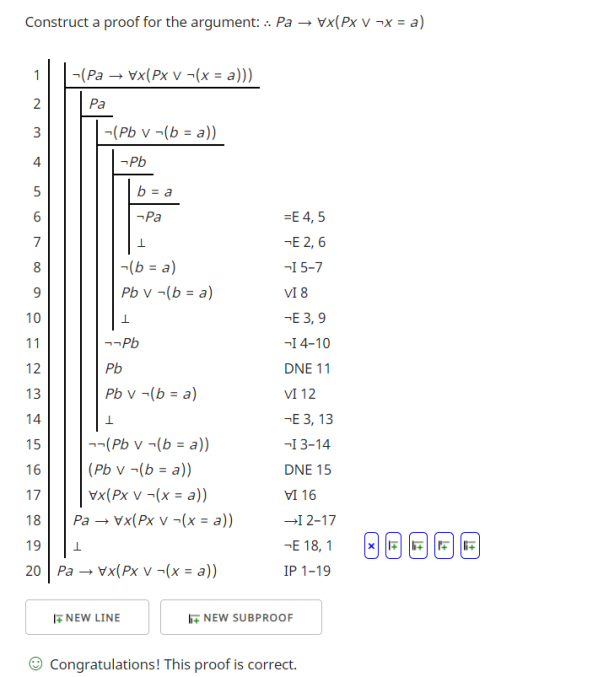
\includegraphics[width=400px, height = 400px]{p2.png}\captionof{figure}{Verification tool returning that my proof is correct for main proof}\end{centering}
\newpage
\begin{flushleft}
Below is the image showing the proof for the derived rule DNE which states that $\neg\neg P = P$.\\
\begin{centering}\hspace*{1pt}\\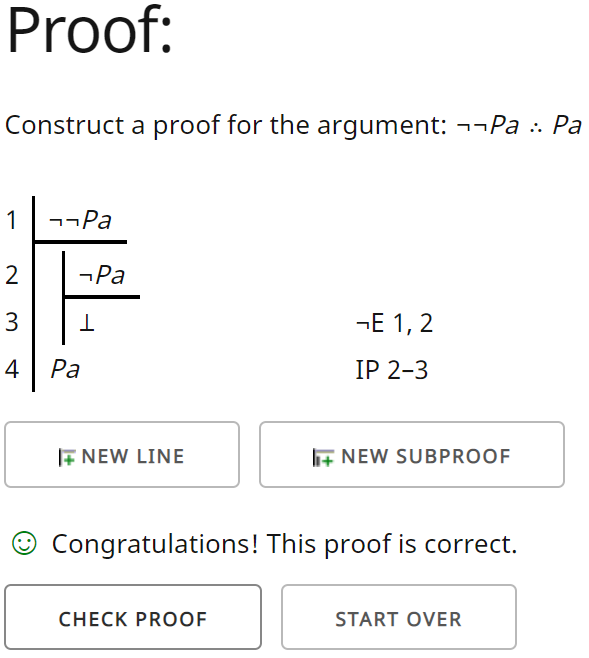
\includegraphics[width=300px, height = 300px]{p1.png}\captionof{figure}{Verification tool returning that my proof of the derived rule DNE is correct}\end{centering}
\end{flushleft}
\newpage
\section{Problem 2}
Recall from Assignment 1 the problem of assigning channels to wifi networks to avoid interference. The
task in this assignment is to set up a logical framework that can handle the same problem in a more
general setting: i.e. with more than two channels and a wider variety of proximity topologies. As before we have some standard requirements:
    \begin{enumerate}[I]
        \item A network uses one, and only one channel.
        \item Networks within close proximity cannot both use the same channel.
        \item “Close proximity” is an anti-reflexive, symmetric relation.
    \end{enumerate}

\begin{enumerate}[(a)]
        \item Carefully define a specification language (that is, a vocabulary or set of propositional variables) necessary to formally specify the requirements laid out above. You may:
        \begin{itemize}
            \item consider the problem in propositional logic or predicate logic;
            \item fix the number of channels and/or networks (e.g. assume there are three channels and four networks).
        \end{itemize}
        \textbf{However}, you will be assessed on how extensible your definitions are – in other words, how easy it is to extend the specification language to cover more general settings (e.g. more channels and/or more networks). \moveToRight{4 marks}\\\\
        Solution: \\
        For this problem i will be defining a specification language in the form of a vocabulary to satisfy the above requirements. To define a vocabulary we need to first define our domain of discourse and our set of: 
        \begin{itemize}
            \item Predicate symbols 
            \item Function symbols
            \item Constant symbols
        \end{itemize}
        our two objects inside our domain of discourse are channels and networks which can be viewed as the following:\\
        Channel:
        \begin{itemize}
            \item Integer id (represents the channel state e.g, 0 = low, 1 = medium, 2 = high)  
        \end{itemize}
        Network:
        \begin{itemize}
            \item String name
            \item Channel connected
            \item List$<$String$>$ close\_proximity\_networks (String was used since it can be the identifier of Network assuming unique naming)
        \end{itemize}
        Using these definitions we can construct the following predicates for our vocabulary:
        
        Network(name, channel,close\_proximity\_networks) which will be used to return true if the tuple values match the entry for the network i.e if the list of close proximity network and channel number match.\fixindent{}
        
        Channel(id) which will be our unary predicate that returns true if the channel with the corresponding id exists, otherwise false.\fixindent{}
        
        is\_close\_proximity(network1, network2) which resolves to true if the two networks are close (the networks are in each others close proximity list) or false if otherwise.\fixindent{}
        
        valid\_channel\_configuration(network1, network2) which will resolves to true if the networks are on different channels (network 1's channel is different to network 2's channel).\\\fixindent{}
        is\_connected(network) which will resolve to true if the network is connected (we can have the channel connected to be -1 before assignment to indicate it is yet to be assigned to a channel.
        
        \fixindent{} Some other unary predicates to restrict our domain of discourse would include:\fixindent{}is\_integer(value) which will be used to make sure valid entries for channel ids.\\is\_String(value) which will be used to make sure valid entries for Network names.\fixindent{}
        
        For this problem it is mostly relational and predicate based so there are no function symbols and constant symbols so these can be considered an empty set so our vocabulary V can be seen as:\\
        V = \{Network, Channel, is\_close\_proximity, valid\_channel\_configuration, is\_connected, is\_integer, is\_String\}\\\fixindent{}
        With this vocabulary we are able to setup a solution to any configuration (if there is one) with n networks and m channels by making sure each network is connected, and making sure each network in close proximity are on different channels.    
%%%%%%%%%%%%%%%%%%%%%%%%%%%%%%%%%%%%%%%%%%%%%%%%%%%%%%%%%%%%%%%%%%%%%%%%%%%%%%%%%%%%%%%%%%%%%        
        \item In your specification language, and subject to the assumptions you have made, define the requirements with logical formulas:
        
        please note for this question i will use the variable X to represent all networks and x to represent individual networks. similarly i will be using the variable Y to represent all channels and y to represent individual networks. a quick explanation of the predicate will also be provided with a quick example aswell for all predicates!
        \begin{enumerate}[(i)]
            \item A network uses one, and only one channel. \moveToRight{2 marks}\\\\
            Solution: \\
            $\psi_1 = \forall x \in X (is\_connected(x))$ \moveToRight{all networks satisfy is\_connected}\\
    
            the following predicate is\_connected(x) can be seen in propositional logic as the following:\\ Assuming there are n channels and $A_x$ represents the proposition that network A is connected to channel x, then we can construct the proposition that a network uses one and only channel in the following:\\
            $\sigma = A_1 \lor A_2 \lor A_3 \lor A_4 \lor ... \lor A_n$ (network is connected to any channel)\\ 
            $\phi_1 = \neg(A_1 \land A_2) \land \neg(A_1 \land A_3) \land ... \land \neg(A_1 \land A_n)$ (no collision on channel 1 but this needs to be done for all combinations) 
            $\phi = \phi_1 \land \phi_2 \land \phi_3 \land ... \land \phi_{n-1}$\\
            so our proposition is\_connected is $\sigma \land \phi$\\\\
            Essentially $\phi$ says that for all possible combinations of connections with collisions we make sure that none of these are true, for example if there were three channels we would say 
            $\phi_1 = \neg(A_1 \land A_2) \land \neg(A_1 \land A_3)$\\
            $\phi_2 = \neg(A_2 \land A_3)$ \moveToRight{note $A_2 \land A_1$ is captured in $\phi_1$}\\
            $\phi = \phi_1 \land \phi_2$\\
            \hspace*{5pt} $= \neg(A_1 \land A_2) \land \neg(A_1 \land A_3) \land \neg(A_2 \land A_3)$\\
            $\sigma$ says that we are connected to any network, so we must be connected to one network, for example if there were three channels we would say\\
            $\sigma = A_1 \lor A_2 \lor A_3$\\ Putting these together we have the predicate function for 3 channels (note this can be extended to m amount of channels\\ $is\_connected(channel) = (channel_1 \lor channel_2 \lor channel_3) \land \neg(channel_1 \land channel_2) \land \neg(channel_1 \land channel_3) \land \neg(channel_2 \land channel_3)$\\\\
            %%%%%%%%%%%%%%%%%%%%%%%%%%%%%%%%%%%%%%%%%%%%%%%%%%%%%%%%%%%%%%%%%%%%%%%%%%%%
            \item Networks within close proximity cannot both use the same channel. \moveToRight{2 marks}\\\\
            Solution: \\
            $\psi_2 = \forall x_1 \in X(\forall x_2 \in X(is\_close\_proximity(x1, x2) \to valid\_configuration(x1, x2)))$\\\\
            We are saying that we will check every network with every other network and for all combinations (nested for loop style) and if two networks are in close proximity that means they are in a valid configuration. by using the same amount of channels as the question above and this time using channel A and channel B which are in close proximity we can set up the propositional formula that if two channels A and B are in close proximity they are on different channels in the following:\\
            $\phi_1 = is\_close\_proximity(A, B)$\\
            let $\phi_2$ be the propositional statement that close proximity networks don't use the same channel. For n amount of networks this can be represented as:\\
            $\phi_2 = \neg(A_1 \land B_1) \land \neg(A_2 \land B_2) \land \neg(A_3 \land B_3) \land ... \land \neg(A_n \land b_n)$\\
            so our requirement $\psi_2$ becomes the following:\\
            $\psi_2 = \phi_1 \to \phi_2$ or in expanded form\\
            $\psi_2 = (is\_close\_proximity(A,B)) \to (\neg(A_1 \land B_1) \land \neg(A_2 \land B_2) \land \neg(A_3 \land B_3) \land ... \land \neg(A_n \land b_n))$\\
            Note is\_close\_proximity(A, B) is simply a predicate which will check if the two networks are close. This predicate formula can also be displayed in code in the following way (Java see next page).\\
            
            \newpage
            Class for channel
            \begin{lstlisting}
public class Channel{

    public int id;
    
    public Channel(int ID){
        this.id = ID;
    }
    
    public int get_Id(){
        return this.id;
    }
}
            \end{lstlisting}
            
            class for Network
            \begin{lstlisting}
import java.util.*;

public class Network{

    public String name;
    public Channel connected;
    public ArrayList<String> close_proximity_networks;
    
    public Network(String name, Channel connected, ArrayList<String> close_proximity_networks){
        this.name = name;
        this.connected = connected;
        this.close_proximity_networks = close_proximity_networks;
    }
    
    public String get_name(){
        return this.name;
    }
    
    public Channel get_channel(){
        return this.connected;
    }
    
    public ArrayList<String> get_close_proximity_networks(){
        return this.close_proximity_networks;
    }
}
            \end{lstlisting}
            
            \newpage
            general solution for this problem and my predicates in code!
            \begin{lstlisting}
import java.util.*;

public class Predicates{

    public ArrayList<Network> all_networks;
    public ArrayList<Channel> all_channels;
    
    public boolean is_close_proximity(Network n1, Network n2){
        //if the network name is apart of the other networks close proximity network list then return true
        if(n1.get_close_proximity_networks().contains(n2.get_name())){
            return true;
        }
        //return false otherwise
        return false;
    }
    
    public boolean valid_configuration(Network n1, Network n2){
        //if the two networks are in close proximity then we check the channels are different to return true
        if(is_close_proximity(n1, n2){
            //both networks use different channels
            return n1.get_channel().get_id() != n2.get_channel().get_id();
        }
        //if the channels are not in close proximity then it is valid eitherway
        return true;
    }
    
    //Now we can construct our final predicate
    public boolean all_configurations_valid(){
        //we want to check all possible configurations
        for(Network n1 : all_networks){
            for(Network n2 : all_networks){
                //anti-reflexive property as this will lead to invalid configuration
                if(n1 == n2){
                    continue;
                }
                //if ANY configuration is invalid we return false as the setup is invalid
                if(!valid_configuration(n1, n2){
                    return false;
                }
            }
        }
        //return true if it does not exit the loop with return false
        return true;
    }
}
                \end{lstlisting}\\
            Note the following predicates for the vocabulary have been defined in the java code above.\\\\
            %%%%%%%%%%%%%%%%%%%%%%%%%%%%%%%%%%%%%%%%%%%%%%%%%%%%%%%%%%%%%%%%%%%%%%%%%%%%%%%
            \item “Close proximity” is an anti-reflexive, symmetric relation. \moveToRight{2 marks}\\\\
            Solution: \\
            $\psi_3 = \forall x1 \in X(\forall x2 \in X(\neg is\_close\_proximity(x1,x1))$\\
            $\psi_4 = \forall x1 \in X(\forall x2 \in X(is\_close\_proximity(x1,x2) \to is\_close\_proximity(x2,x1))$\\\\
            $\psi_3$ is the logical formula which states for all networks inside our network domain, they cannot be in close proximity with themselves which is an anti-reflexive relation.\\\\
            $\psi_4$ is the logical formula which states for all networks if network A is in close proximity to network B, then that also implies network B is in close proximity with network A which a symmetric relation.\\\\
            "Close proximity" must be an anti-reflexive and symmetric relation in order for valid configurations. This is because if a Network can be in close proximity with itself that means the valid\_configuration would return false since it will show up as both networks using the same channel even though its the same network. "close proximity" must also be a symmetric relation, since if A is in close proximity with B, that means B must be in close proximity with A. The above formulas slightly modify the code we have written above the following\\
            re-defining the code to allow close\_proximity to be an anti-reflexive and symmetric. Please also anti-reflexive was implemented in the above code in the all\_valid\_
            \begin{lstlisting}
public boolean is_close_proximity(Network n1, Network n2){
    //anti-reflexive property by not letting n1 = n2 be true
    //i.e. if the two networks are the same return false!
    if(n1 == n2){
        return false;
    }
    //adding the symmetric relation by making n1 close proximity to n2
    if(n2.get_close_proximity_networks().contains(n1.get_name())){
        return true;
    }
    //if the network name is apart of the other networks close proximity network list then return true
    if(n1.get_close_proximity_networks().contains(n2.get_name())){
        return true;
    }
    //return false otherwise
    return false;
}
            
            
            
            
            
//this allows use to now modify all_valid configuration to the following
//since we now have anti-reflexive inside our close proximity rather than in the predicate all_configurations_valid we can just simply call valid_configuration(n1,n2)
public boolean all_configurations_valid(){
        //we want to check all possible configurations
        for(Network n1 : all_networks){
            for(Network n2 : all_networks){
                //if ANY configuration is invalid we return false as the setup is invalid
                if(!valid_configuration(n1, n2){
                    return false;
                }
            }
        }
        //return true if it does not exit the loop with return false
        return true;
}
            \end{lstlisting}
            
        \end{enumerate}
        Note that since we have "close proximity" as a symmetric relation, that means if network A is inside of network B's close proximity list, that also means that network B is also inside of network A's close proximity list, this can be shown in code with the following to truly show the symmetric property.
        
        \begin{lstlisting}
//suppose this is the method for making two networks within close proximity
public void make_close_proximity(Network A, Network B){
    //this shows the symmetry since A is close proximity to B
    //also means B is close proximity to A
    //since we make them BOTH close proximity to each other.
    A.get_close_proximity_networks.add(B.get_name());
    B.get_close_proximity_networks().add(A.get_name());
}
        \end{lstlisting}.
        \newpage
        \begin{flushleft}
            Consider the following set-up: we have exactly three channels: hi, med, lo; and (at least) four networks Alpha, Bravo, Charlie, Delta with close proximity as defined in the following diagram:
        \end{flushleft}

        \begin{centering}\hspace*{1pt}\\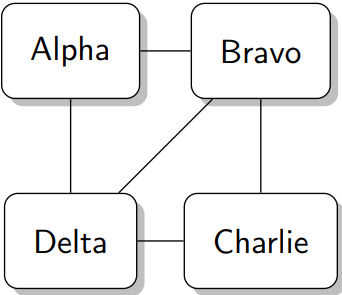
\includegraphics[width=100px, height = 100px]{network2.png}\captionof{figure}{Network configuration between all four networks and three channels}\end{centering}
        We now want to refine our specification (i.e. add requirements) so that any model which satisfies all the requirements will necessarily have the structure detailed here.
        
        \item  Extending your specification language if necessary, provide a set of requirements which, together with your answer to (b), ensures any satisfying model has the structure detailed here. \moveToRight{10 marks}\\\\
        Solution: \\
        Since in part (b) we gave requirements for a more general solution which will solve for any configuration (if there is a solution) we simply have to just add requirements so that all models have the structure shown in Figure 3. The following extra requirements can be added to achieve this:
        \begin{enumerate}[(1)]
            \item we have 4 networks and 3 channels
            \item two UNIQUE networks are in "close proximity" to every other network
            \item the other two networks are ONLY in close proximity to the networks in (2)
        \end{enumerate}
        By saying that the set of all networks is X and the set of all channels is Y
        these requirements can be shown in predicate formulas in the following:
                \begin{enumerate}[(1)]
            \item $\psi_5 = (|X| = 4) \land (|Y| = 3)$\\
            This essentially says that the size of our network set is 4 and the size of our channel set is 3
            \item $\psi_6 = (x1,n1 \exists X(\forall x2 \in X (is\_close\_proximity(x1, x2) \land (is\_close\_proximity(n1,x2)))  \land \\\neg(x1 = x2)$\\
            This essentially says that there exists two networks x1 and x2 in the set of networks which is in close proximity to ALL other networks and those two networks are not the same network. 
            \item $\psi_7 = (x1,n1 \exists X(\forall x2 \in X (is\_close\_proximity(x1, x2) \land (is\_close\_proximity(n1,x2)))  \land \\\neg(x1 = x2) (u1, u2 \exists X(is\_close\_proximity(u1, x1) \land is\_close\_proximity(u1, n1) \land \\ is\_close\_proximity(u2, x1) \land is\_close\_proximity(u2, n1) \land \\\neg is\_close\_proximity(u1, u2) \land \neg(u1 = u2)$\\
            This seems like a much more complicated predicate formula, however this is because we needed to write out $\psi_6$ to reference the networks x1 and n1, essentially it states that two networks are in close proximity to all other networks and that there are two distinct networks u1 and u2 that are in close proximity to those networks and not in close proximity to each other and they are not the same network.
        \end{enumerate}
        \\We will name our predicates $\psi_5$ $\psi_6$ $\psi_7$ as correct\_sizes, two\_connected\_to\_all and two\_unique\_connected respectively
        These new requirements can also be added to the previous predicates $\psi_{1-4}$ to give us our final requirement $\psi$ as:\\
        $\psi = \psi_1 \land \psi_2 \land \psi_3 \land \psi_4 \land \psi_5 \land \psi_6 \land \psi_7$\\
        This can also be shown in the code above in part (b) along with the following additions below to introduce our new requirements note all this code is being added to the Predicates class in the code.
        \begin{lstlisting}
//we will also be adding new class variables
public Network connected_to_all1 = null;
public Network connected_to_all2 = null;
public Network uniq1 = null;
public Network uniq2 = null;
public boolean correct_sizes(){
    return (all_networks.size() == 4 && all_channels.size() == 3);
}
//our predicate to make sure we have only two networks which are in close proximity to all other networks
public boolean two_connected_to_all(){
    //this flag will be used to be a check if the network is
    //in close proximity to all other networks
    //if a network is not in close proximity to any network we want to go to the next
    //network as this one is not connected to ALL networks. we reset the flag at each iteration
    //if the flag is false.
    boolean flag = true;
    //count how many networks are connected to ALL networks
    int count = 0;
    //scan through all combinations of the networks
    for(Network n1 : all_networks){
        for(Network n2 : all_networks){
            //if n1 is not in close proximity to all other networks we want to set flag as false
            //and go to the next network
            if(!is_close_proximity(n1, n2) && n1 != n2){
                flag = false;
                break;
            }
        }
        //if the flag is false that means we dont want to increase the counter or update
        //our class vairables
        if(flag == false){
            flag = true;
            continue;
        }
        //otherwise we want to set the class variables in order
        if(connected_to_all2 == null && connected_to_all1 != null){
            connected_to_all2 = n1;
        }

        if(connected_to_all1 == null){
            connected_to_all1 = n1;
        }
        //and increment the count
        count++;
    }
    //return the statement that the count must be exactly 2
    //and that the two networks connected to all the other networks
    //are not the same network
    return (count == 2) && (connected_to_all1 != connected_to_all2);
}

//our predicate to make sure that the other two networks are also connected to the other networks
//that connect to everything and are not connected to any other node
public boolean two_unique_connected(){
    //if we don't have two networks which are connected to all other networks
    if(null == connected_to_all1 || null == connected_to_all2) {
        return false;
    }
    //otherwise we want to isolate the other 2 networks and make sure they are
    //1. connected to the connected_to_all networks AND
    //2. those two networks are not connected to each other
    //3. those two networks are not the same network
    Network n1 = null;
    Network n2 = null;
    //find the two networks which are not the ones connected to the rest of the networks
    for(Network n : all_networks){
        if(n1 != null && (n != connected_to_all1 && n != connected_to_all2) && n2 == null){
            n2 = n;
        }
        if((n != connected_to_all1 || n != connected_to_all2) && n1 == null){
            n1 = n;
        }
    }
    //if those two networks are NOT in close proximity with ONLY the two networks that are connected
    //to the rest, we return false
    if(n1.get_close_proximity_networks().size() != 2 && n2.get_close_proximity_networks().size() != 2){
        return false;
    }
    //if those two networks are in close proximity to each other
    //return false
    if(is_close_proximity(n1, n2)){
        return false;
    }
    //if the network is not in close proximity with the two networks
    //connected to the all networks, return false
    if(!n1.get_close_proximity_networks().contains(connected_to_all2.get_name()) &&
            !n1.get_close_proximity_networks().contains(connected_to_all1.get_name())){
        return false;
    }
    if(!n2.get_close_proximity_networks().contains(connected_to_all2.get_name()) &&
            !n2.get_close_proximity_networks().contains(connected_to_all1.get_name())) {
        return false;
    }
    //otherwise return true since it has passed all checks
    unique1 = n1;
    unique2 = n2;
    return true;
}
    \end{lstlisting}
    With our new predicates which restrict all models to the configuration in Figure 3 we can finally modify all\_configurations\_valid which achieved $\psi$ in the following code
    \begin{lstlisting}
//this allows use to now modify all_valid configuration to the following
//since we now have anti-reflexive inside our close proximity rather than in the predicate all_configurations_valid we can just simply call valid_configuration(n1,n2)
public boolean all_configurations_valid(){
    //we want to check all possible configurations
    for(Network n1 : all_networks){
        for(Network n2 : all_networks){
            //if ANY configuration is invalid we return false as the setup is invalid
            if(!valid_configuration(n1, n2)){
                return false;
            }
        }
    }
    //return true if it does not exit the loop with return false
    return correct_sizes() && two_connected_to_all() && two_unique_connected();
}
        \end{lstlisting}
        from these predicates we can also make the observation that since two networks are connected to every other networks, those networks must run on different channels, and since the other two networks are not connected to each other, they must run on the same channel (this will be proven in (c) and (d). The following is a satisfying model to this problem. 
        \begin{enumerate}
            \item A = channel medium
            \item B = channel High
            \item C = channel medium
            \item D = channel low
        \end{enumerate}
        \newpage
        When this is run with the following test code giving the same configuration, we receive the following output
        \begin{lstlisting}
import java.util.*;

public class test {
    public static void main(String args[]) {
        Channel low = new Channel(0);
        Channel medium = new Channel(1);
        Channel high = new Channel(2);

        ArrayList<String> close_proximity_to_a = new ArrayList<String>();
        close_proximity_to_a.add("B");
        close_proximity_to_a.add("D");
        Network A = new Network("A", medium, close_proximity_to_a);

        ArrayList<String> close_proximity_to_b = new ArrayList<String>();
        close_proximity_to_b.add("A");
        close_proximity_to_b.add("C");
        close_proximity_to_b.add("D");
        Network B = new Network("B", high, close_proximity_to_b);

        ArrayList<String> close_proximity_to_c = new ArrayList<String>();
        close_proximity_to_c.add("B");
        close_proximity_to_c.add("D");
        Network C = new Network("C", medium, close_proximity_to_c);

        ArrayList<String> close_proximity_to_d = new ArrayList<String>();
        close_proximity_to_d.add("A");
        close_proximity_to_d.add("B");
        close_proximity_to_d.add("C");
        Network D = new Network("D", low, close_proximity_to_d);

        ArrayList<Channel> channels = new ArrayList<Channel>();
        channels.add(low);
        channels.add(medium);
        channels.add(high);

        ArrayList<Network> networks = new ArrayList<Network>();
        networks.add(A);
        networks.add(B);
        networks.add(C);
        networks.add(D);

        Predicates check = new Predicates(networks, channels);
        System.out.println("Correct size of configuration 4 networks 3 channels- : " + check.correct_sizes());
        System.out.println("Only two networks connected to all other networks: " + check.two_connected_to_all());
        System.out.println("Two networks connected to the ones above but not to each other: " + check.two_unique_connected());
        
        System.out.println("Final valid configuration (main requirements): " + check.all_configurations_valid());
        System.out.println("A connected to : " + A.get_close_proximity_networks());
        System.out.println("B connected to : " + B.get_close_proximity_networks());
        System.out.println("C connected to : " + C.get_close_proximity_networks());
        System.out.println("D connected to : " + D.get_close_proximity_networks());
        System.out.println("The two channels which were connected to all other channels satisfying psi_6 are : "
                + check.connected_to_all1.get_name() + " and "
                + check.connected_to_all2.get_name());
        System.out.println("The two channels which are unique satisfying psi_7 are : " 
                + check.unique1.get_name() + " and " + check.unique2.get_name());
        
    }
}

        \end{lstlisting}
        when the above code is run we get the following output
        \begin{centering}\hspace*{1pt}\\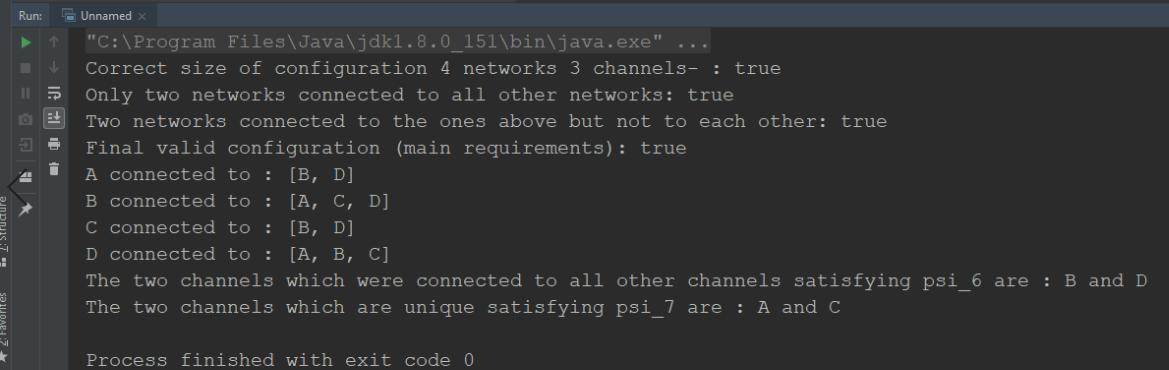
\includegraphics[width=400px, height = 200px]{output3.png}\captionof{figure}{code output with the configuration above with same structure in Figure 3}\end{centering}
        
        Note this code produces the correct output and can be copied and pasted from above, and tested with different values, i did not use the predicate make\_close\_proximity in my testing as i already made close proximity with the symmetric nature by adding both networks in close proximity to each other's close proximity list.
        \newpage
        \item How would you use a SAT-solver (for First Order Logic) such as Z3 or IDP to show that in any model satisfying your requirements, Alpha and Charlie use the same channel? \moveToRight{5 marks}\\\\
        Solution:\\
        Similair to the lecture example for solving a simpler version of the zebra puzzle, i would load each of my variables in, so each channel will be loaded in as integers, and i would set these channels to set values, so high = 2, medium = 1 and low = 0. Then i would load in my Networks as integers which range from 0-2 (indicating their channels). Then i would assert the conditions that for my defined close proximity networks that they cannot have equal values. So in the defined model above, we have the following:\\
        \begin{itemize}
            \item Alpha != Bravo
            \item Alpha != Delta
            \item Bravo != Alpha
            \item Bravo != Charlie
            \item Bravo != Delta
            \item Charlie != Bravo
            \item Charlie != Delta
            \item Delta != Alpha
            \item Delta != Bravo
            \item Delta != Charlie
        \end{itemize}
        all these conditions enforce the close proximity in the given
        \begin{itemize}
            \item Alpha is in close proximity to Bravo and Delta
            \item Bravo is in close proximity to Alpha, Charlie and Delta
            \item Charlie is in close proximity to Bravo and Delta
            \item Delta is in close proximity to Alpha, Bravo and Charlie
        \end{itemize}
        which follows our structure in Figure 3 as we are also using 3 channels low, medium and high. 
        after we would try to get all models by adding more conditions and exhausting all possibilities to verify that all satisfying models have Alpha and Charlie on the same Network.\\\\ to get all models i would first run it with those conditions in place, then after i check satisfiability and get the model, we will now make it so alpha cannot be channel 0 and repeat till we have exhausted all possible channels giving all possible models. \\\\ This will also what i will be using for the bonus to implement the solution using Z3.
        \newpage
        \textbf{Bonus:} Implement your solution to the previous question in a SAT-solver to show that in any model satisfying the requirements, Alpha and Charlie use the same channel. Either include a link to your solution or provide the code so it can be easily copy-pasted and run. \moveToRight{10* marks}\\\\
        Solution:\\
        \z3{
            (assert)
        }
        
\end{enumerate}

\end{document}
